\section{Interferencia de doble rendija en \(T^2_{27}\): memoria de camino, regla de Born y unitariedad dodecafásica}
\label{sec:md-sucesora-interferometria-t27}

La realización finita se construye sobre
\[
 \mathcal H_{\mathrm{cam}}
 =\ell^2\!\left(T_{27}^{2}\right)\otimes\mathbb C^4,
 \qquad
 T_{27}^{2}=(\mathbb Z/27\mathbb Z)^2,
\]
donde el factor de dimensión \(4\) registra las direcciones
\((N,S,E,W)\). La memoria explícita de la trayectoria añade el factor
\(\mathbb C^2_{\mathrm{mem}}\). El paso microscópico es el operador
\begin{equation}
 U_{\mathrm{micro}}=S D_J C_4,
 \label{eq:md-sucesora-interferometro-microstep}
\end{equation}
con \(C_4\) unitario, \(D_J\) diagonal y \(S\) como desplazamiento condicionado
por la dirección. En consecuencia,
\[
 U_{\mathrm{micro}}^*U_{\mathrm{micro}}=I,
\]
y la norma se conserva en cada paso.

\subsection{Preparación de las \(2\) trayectorias y pantalla de lectura}

Las dos aperturas se fijan en
\[
 (x_0,y_1)=(2,8),
 \qquad
 (x_0,y_2)=(2,18),
\]
con el mismo estado direccional inicial. Si \(\psi_1\) y \(\psi_2\) son las
amplitudes propagadas desde cada apertura, la pantalla situada en \(x=24\)
publica, para un solapamiento real de memoria \(\mu\in[0,1]\),
\begin{equation}
 I_\mu(y)
 =\frac12\sum_d
 \left(
  |\psi_1(24,y,d)|^2+|\psi_2(24,y,d)|^2
  +2\operatorname{Re}\!\left[
   \mu\,\overline{\psi_1(24,y,d)}\psi_2(24,y,d)
  \right]
 \right).
 \label{eq:md-sucesora-interferometro-intensidad}
\end{equation}
La fórmula se obtiene también introduciendo los marcadores
\[
 |m_1\rangle=(1,0),
 \qquad
 |m_2\rangle=(\mu,\sqrt{1-\mu^2})
\]
y trazando \(\mathbb C^2_{\mathrm{mem}}\). Esta igualdad identifica el
solapamiento de los registros, no una pérdida de norma, como origen de la
atenuación de las franjas. En particular,
\begin{equation}
 \mathcal V(\mu)=|\mu|\,\mathcal V(1).
 \label{eq:md-sucesora-interferometro-visibilidad}
\end{equation}
Para \(\mu=0\), una corrección de fase no puede reconstruir el término cruzado;
si los marcadores se deshacen unitariamente antes de la recombinación, se
recupera exactamente la curva \(\mu=1\).

\subsection{Identidades de unitariedad del orden dodecafásico bajo un presupuesto común de amplitud}

El bloque de control consta de \(12\) pulsos orientados y suma vectorial nula.
Los \(6\) primeros se obtienen de una semilla direccional mediante la firma
dodecafásica; los \(6\) restantes son sus opuestos. Se comparan cuatro
secuencias de \(36\) pasos:
\begin{enumerate}
 \item la secuencia canónica, repetida durante \(3\) ciclos completos;
 \item su inversión orientada;
 \item una secuencia en la que un par opuesto se sustituye por fases comunes
       de la misma norma;
 \item una permutación aleatoria del mismo multiconjunto de pulsos.
\end{enumerate}
Todas conservan el número de pulsos, la suma vectorial nula y el presupuesto
cuadrático. La diferencia entre sus patrones mide, por tanto, la dependencia
respecto del orden no conmutativo y de la información direccional, no una
inyección desigual de norma o energía.

La no conmutatividad se verifica sobre un estado sonda fijado antes de la
lectura:
\[
 \left\|U_bU_a\psi-U_aU_b\psi\right\|_2
 =0.24776388825652637.
\]
El control numérico proporciona
\[
 \|C_4^*C_4-I\|_{\max}=0,
 \qquad
 \max_t\bigl|\|\psi_t\|_2^2-1\bigr|
 =1.3322676295501878\times10^{-15},
\]
\[
 \Delta B_2=2.220446049250313\times10^{-16},
 \qquad
 \varepsilon_{\mathrm{Born}}
 =1.734723475976807\times10^{-18},
\]
\[
 \varepsilon_{\mathcal V(\mu)}
 =2.220446049250313\times10^{-16},
\]
donde \(\Delta B_2\) es la dispersión máxima del presupuesto cuadrático entre
las cuatro secuencias.

\begin{table}[tbp]
\centering
\caption{Interferencia y distancia respecto de la secuencia canónica después de \(36\) pasos.}
\label{tab:md-sucesora-interferometro-resultados}
\begin{tabular}{lccc}
\toprule
Secuencia & \(\mathcal V_{\mathrm{lineal}}\) &
distancia de variación total & fidelidad media \\
\midrule
canónica      & \(0.5992212256\) & \(0\)            & \(1.0000000000\) \\
inversa       & \(0.5974219552\) & \(0.0333923142\) & \(0.9740951119\) \\
par sustituido& \(0.5907431085\) & \(0.0628288605\) & \(0.9417893564\) \\
aleatorizada  & \(0.6254301808\) & \(0.0963185652\) & \(0.6564185376\) \\
\bottomrule
\end{tabular}
\end{table}

\subsection{Interferencia reconstruida en \(T^2_{27}\): distribución de detección y dominio físico}

\begin{theorem}[Interferencia unitaria con memoria explícita de camino]
Para la dinámica definida por \eqref{eq:md-sucesora-interferometro-microstep},
la intensidad obtenida al trazar el registro de camino coincide con
\eqref{eq:md-sucesora-interferometro-intensidad}; la visibilidad satisface
\eqref{eq:md-sucesora-interferometro-visibilidad}; y secuencias con idéntico
presupuesto cuadrático pueden producir patrones distintos cuando difiere su
orden.
\end{theorem}

La demostración es finita: unitariedad de cada factor, expansión del cuadrado
de la suma de las dos ramas y contracción parcial del marcador. Los controles
numéricos anteriores verifican la ejecución sobre \(T_{27}^{2}\). La carta
concreta que lleva el estado dodecafásico a fases direccionales constituye una
realización física declarada; no se identifica por definición con el retorno
temporal de \(108\) fases. La escala electrónica se aplica después de la
dinámica adimensional y no selecciona la palabra ni ajusta las franjas.

La realización quedaría refutada por pérdida de unitariedad, discrepancia entre
la memoria explícita y la regla de Born, creación de interferencia por una fase
cuando \(\mu=0\), dependencia del presupuesto energético entre secuencias o uso
del resultado de la pantalla para escoger retrospectivamente el orden de los
pulsos.

\begin{figure}[tbp]
\centering
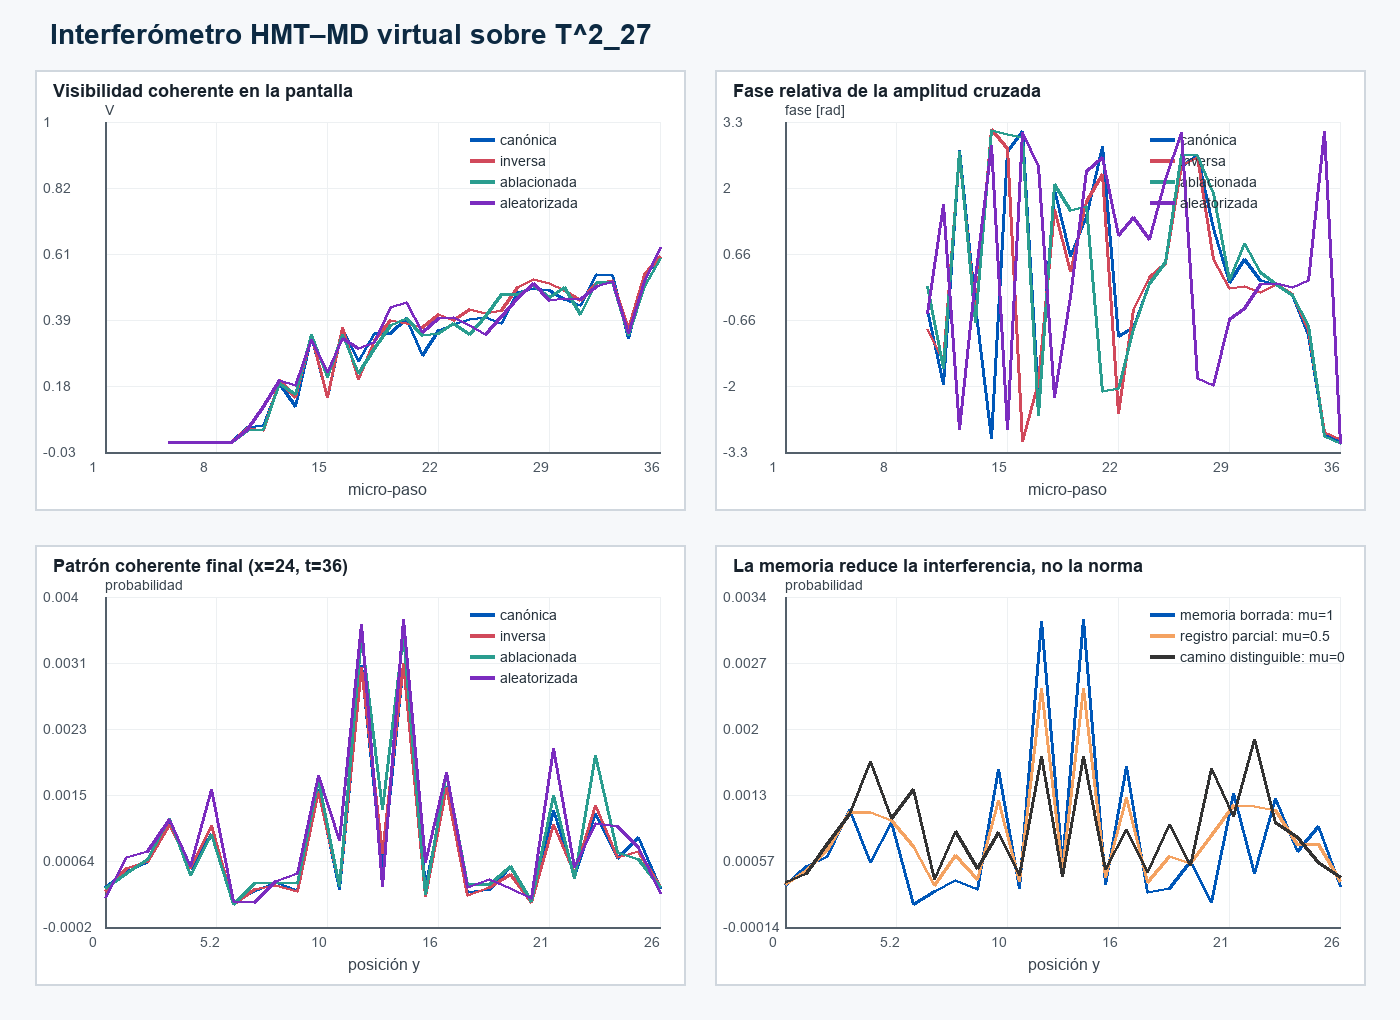
\includegraphics[width=.96\linewidth]{figures/parte_iv/01_curvas_y_patrones.png}
\caption{Evolución de la visibilidad, fase relativa y patrón final para las cuatro secuencias con presupuesto común.}
\label{fig:md-sucesora-interferometro-patrones}
\end{figure}

\begin{figure}[tbp]
\centering
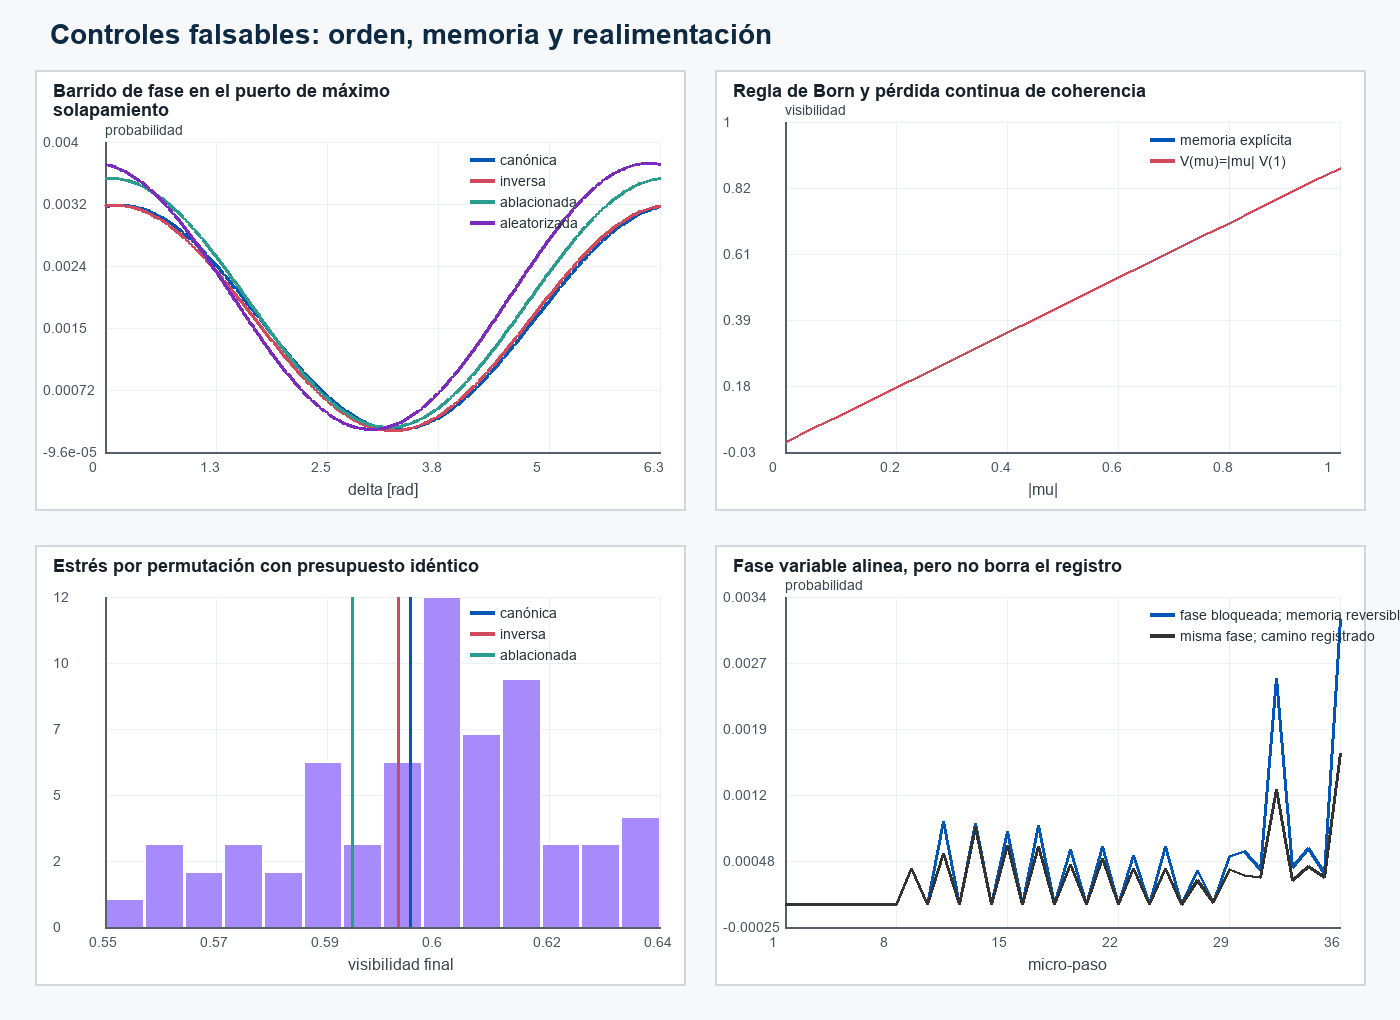
\includegraphics[width=.96\linewidth]{figures/parte_iv/02_estres_memoria_y_control.png}
\caption{Controles de orden, memoria de camino y realimentación de fase.}
\label{fig:md-sucesora-interferometro-controles}
\end{figure}
